\exercisesheader{}

% 1

\eoce{\qt{Fill in the blank\label{fitb_anova}} When doing an ANOVA, you observe 
large differences in means between groups. Within the ANOVA framework, this 
would most likely be interpreted as evidence strongly favoring the \underline{\hspace{20mm}} hypothesis.
}{}

% 2

\eoce{\qtq{Which test\label{which_test_anova}} We would like to test if 
students who are in the social sciences, natural sciences, arts and 
humanities, and other fields spend the same amount of time studying for 
this course. What type of test should we use? Explain your reasoning.
}{}

% 3

\eoce{\qt{Chicken diet and weight, Part III\label{chick_wts_anova}} In Exercises~\ref{chick_wts_linseed_horsebean} and \ref{chick_wts_casein_soybean} we compared the effects of two types of feed at a time. A better analysis would first consider all feed types at once: casein, horsebean, linseed, meat meal, soybean, and sunflower. The ANOVA output below can be used to test for differences between the average weights of chicks on different diets.
\begin{center}
\begin{tabular}{lrrrrr}
\hline
        & Df    & Sum Sq        & Mean Sq   & F value   & Pr($>$F) \\ 
\hline
feed        & 5     & 231,129.16    & 46,225.83     & 15.36     & 0.0000 \\ 
Residuals   & 65 & 195,556.02   & 3,008.55  &       &  \\ 
\hline
%\multicolumn{6}{r}{$s_{pooled} = 55.85$ on $df=65$}
\end{tabular}
\end{center}
Conduct a hypothesis test to determine if these data provide convincing evidence that the average weight of chicks varies across some (or all) groups. Make sure to check relevant conditions. Figures and summary statistics are shown below.

\begin{minipage}[c]{0.65\textwidth}
\begin{center}
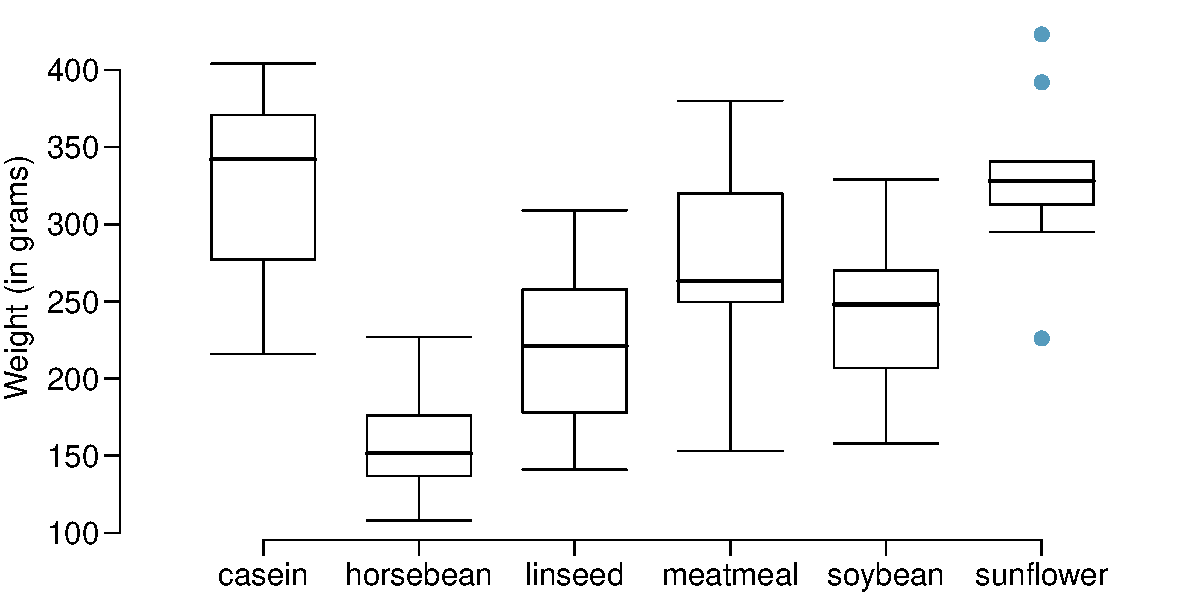
\includegraphics[width= \textwidth]{ch_inference_for_means/figures/eoce/chick_wts_anova/chick_wts_box.pdf}
\end{center}
\end{minipage}
\begin{minipage}[c]{0.35\textwidth}
{\footnotesize\begin{tabular}{l c c c}
\hline
            & Mean      & SD        & n \\
\hline
casein          & 323.58        & 64.43 & 12 \\
horsebean   & 160.20        & 38.63 & 10 \\
linseed         & 218.75        & 52.24 & 12 \\
meatmeal    & 276.91        & 64.90 & 11 \\
soybean         & 246.43        & 54.13 & 14 \\
sunflower       & 328.92        & 48.84 & 12 \\
\hline
\end{tabular}}
\end{minipage}
}{}

% 4

\eoce{\qt{Teaching descriptive statistics\label{teach_descriptive_stats}} A study 
compared five different methods for teaching descriptive statistics. The five 
methods were traditional lecture and discussion, programmed textbook 
instruction, programmed text with lectures, computer instruction, and computer 
instruction with lectures. 45 students were randomly assigned, 9 to each 
method. After completing the course, students took a 1-hour exam. 
\begin{parts}
\item What are the hypotheses for evaluating if the average test scores are 
different for the different teaching methods?
\item What are the degrees of freedom associated with the $F$-test for 
evaluating these hypotheses?
\item Suppose the p-value for this test is 0.0168. What is the conclusion?
\end{parts}
}{}

% 5

\eoce{\qt{Coffee, depression, and physical activity\label{coffee_depression_phys_act}} 
Caffeine is the world's most widely used stimulant, with approximately 80\% consumed 
in the form of coffee. Participants in a study investigating the relationship between 
coffee consumption and exercise were asked to report the number of hours they spent per 
week on moderate (e.g., brisk walking) and vigorous (e.g., strenuous sports and jogging) 
exercise. Based on these data the researchers estimated the total hours of metabolic 
equivalent tasks (MET) per week, a value always greater than 0. The table below gives 
summary statistics of MET for women in this study based on the amount of coffee consumed.
\footfullcite{Lucas:2011}
 
\begin{adjustwidth}{-4em}{-4em}
\begin{center}
\begin{tabular}{l  r  r  r  r  r  r}
                & \multicolumn{5}{c}{\textit{Caffeinated coffee consumption}} \\
\cline{2-6}
                & $\le$ 1 cup/week  & 2-6 cups/week & 1 cup/day 
                                            & 2-3 cups/day  & $\ge$ 4 cups/day  & Total \\
\hline
Mean            & 18.7              & 19.6          & 19.3  
                                            & 18.9          & 17.5 \\
SD              & 21.1              & 25.5          & 22.5  
                                            & 22.0          & 22.0 \\
n               & 12,215            & 6,617         & 17,234    
                                            & 12,290        & 2,383             & 50,739 \\
\hline
\end{tabular}
\end{center}
\end{adjustwidth}

\begin{parts}

\item Write the hypotheses for evaluating if the average physical activity level 
varies among the different levels of coffee consumption.

\item Check conditions and describe any assumptions you must make to proceed with 
the test.

\item Below is part of the output associated with this test. Fill in the empty cells.

\begin{center}
\renewcommand{\arraystretch}{1.25}
\begin{tabular}{lrrrrr}
  \hline
            & Df
                        & Sum Sq
                                    & Mean Sq
                                                & F value
                                                            & Pr($>$F) \\ 
  \hline
coffee      & \fbox{\textcolor{white}{{\footnotesize XXXXX}}}    
                        & \fbox{\textcolor{white}{{\footnotesize XXXXX}}}      
                                    & \fbox{\textcolor{white}{{\footnotesize XXXXX}}}           
                                                & \fbox{\textcolor{white}{{\footnotesize XXXXX}}}
                                                            & 0.0003 \\ 
Residuals   & \fbox{\textcolor{white}{{\footnotesize XXXXX}}} 
                        & 25,564,819
                                    & \fbox{\textcolor{white}{{\footnotesize  XXXXX}}}
                                                &
                                                            &  \\ 
   \hline
Total       & \fbox{\textcolor{white}{{\footnotesize XXXXX}}} 
                        & 25,575,327
\end{tabular}
\end{center}

\item What is the conclusion of the test?

\end{parts}
}{}

% 6

\eoce{\qt{Student performance across discussion sections\label{student_performance_sections}} A professor who teaches a large introductory statistics class (197 students) with eight discussion sections would like to test if student performance differs by discussion section, where each discussion section has a different teaching assistant. The summary table below shows the average final exam score for each discussion section as well as the standard deviation of scores and the number of students in each section.
\begin{center}
\begin{tabular}{rrrrrrrrr}
  \hline
            & Sec 1 & Sec 2 & Sec 3 & Sec 4 & Sec 5 & Sec 6 & Sec 7 & Sec 8 \\ 
  \hline
$n_i$       & 33 & 19 & 10 & 29 & 33 & 10 & 32 & 31 \\ 
$\bar{x}_i$ & 92.94 & 91.11 & 91.80 & 92.45 & 89.30 & 88.30 & 90.12 & 93.35 \\ 
$s_i$       & 4.21 & 5.58 & 3.43 & 5.92 & 9.32 & 7.27 & 6.93 & 4.57 \\ 
   \hline
\end{tabular}
\end{center}
The ANOVA output below can be used to test for differences between the average scores from the different discussion sections.
\begin{center}
\begin{tabular}{lrrrrr}
\hline
            & Df        & Sum Sq & Mean Sq  & F value & Pr($>$F) \\ 
\hline
section         & 7         & 525.01    & 75.00         & 1.87  & 0.0767 \\ 
Residuals   & 189   & 7584.11   & 40.13         &       &  \\ 
\hline
\end{tabular}
\end{center}
Conduct a hypothesis test to determine if these data provide convincing evidence that the average score varies across some (or all) groups. Check conditions and describe any assumptions you must make to proceed with the test.
}{}

% 7

\eoce{\qt{GPA and major\label{gpa_major}} Undergraduate students taking an introductory statistics course at Duke University conducted a survey about GPA and major. The side-by-side box plots show the distribution of GPA among three groups of majors. Also provided is the ANOVA output.
\begin{center}
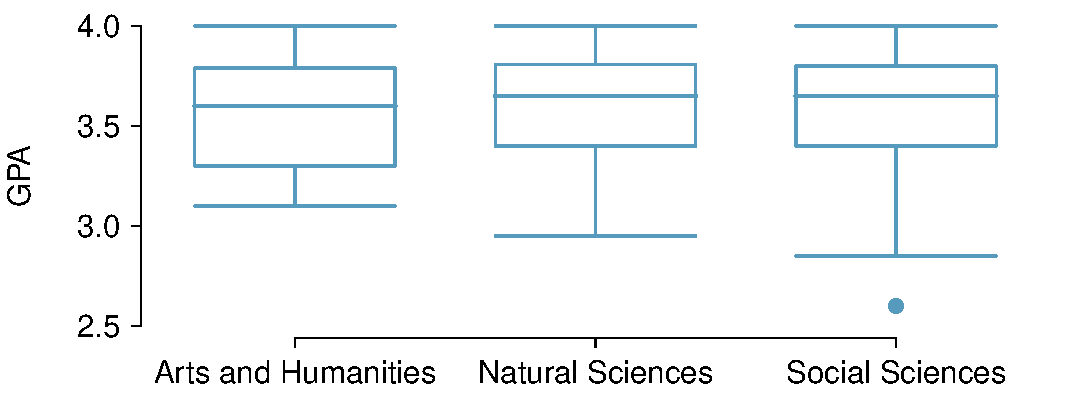
\includegraphics[width=0.85\textwidth]{ch_inference_for_means/figures/eoce/gpa_major/gpa_major.pdf}
\end{center}
\begin{center}
\begin{tabular}{lrrrrr}
  \hline
            & Df    & Sum Sq    & Mean Sq   & F value   & Pr($>$F) \\ 
  \hline
major       & 2     & 0.03      & 0.015      & 0.185     & 0.8313 \\ 
Residuals   & 195   & 15.77     & 0.081      &           &  \\ 
   \hline
\end{tabular}
\end{center}
\begin{parts}
\item Write the hypotheses for testing for a difference between average GPA across majors.
\item What is the conclusion of the hypothesis test?
\item How many students answered these questions on the survey, i.e. what is the sample size?
\end{parts}
}{}

% 8

\eoce{\qt{Work hours and education\label{work_hours_education}} The General Social Survey 
collects data on demographics, education, and work, among many other characteristics 
of US residents. \footfullcite{data:gss} Using ANOVA, we can consider 
educational attainment levels for all 1,172 respondents at once. Below are the 
distributions of hours worked by educational attainment and relevant summary 
statistics that will be helpful in carrying out this analysis.
\begin{center}

\begin{tabular}{l  r  r  r  r  r  r}
                & \multicolumn{5}{c}{\textit{Educational attainment}} \\
\cline{2-6}
                & Less than HS  & HS    & Jr Coll   & Bachelor's & Graduate & Total \\
\hline
Mean            & 38.67         & 39.6  & 41.39     & 42.55     & 40.85     & 40.45 \\
SD              & 15.81         & 14.97 & 18.1      & 13.62     & 15.51     & 15.17 \\
n               & 121           & 546   & 97        & 253       & 155       & 1,172 \\
\hline
\end{tabular}

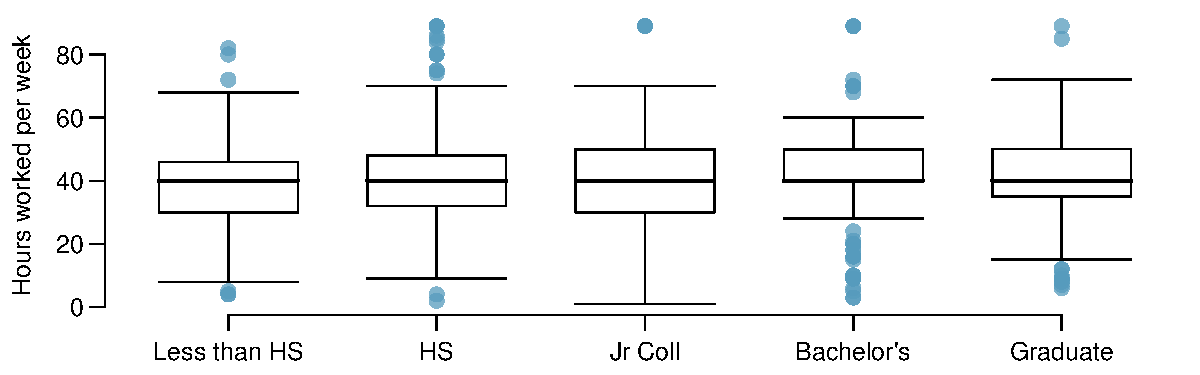
\includegraphics[width=\textwidth]{ch_inference_for_means/figures/eoce/work_hours_education/work_hours_education.pdf}
\end{center}
\begin{parts}
\item Write hypotheses for evaluating whether the average number of hours 
worked varies across the five groups.
\item Check conditions and describe any assumptions you must make to proceed 
with the test.
\item Below is part of the output associated with this test. Fill in the 
empty cells.

\begin{center}
\renewcommand{\arraystretch}{1.25}
\begin{tabular}{lrrrrr}
  \hline
            & Df    
                    & Sum Sq        
                            & Mean Sq       
                                    & F-value      
                                            & Pr($>$F) \\ 
  \hline
degree      & \fbox{\textcolor{white}{{\footnotesize XXXXX}}}       
                    & \fbox{\textcolor{white}{{\footnotesize XXXXX}}}       
                            & 501.54    
                                    & \fbox{\textcolor{white}{{\footnotesize XXXXX}}}   
                                            & 0.0682 \\ 
Residuals   & \fbox{\textcolor{white}{{\footnotesize XXXXX}}} 
                    & 267,382     
                            & \fbox{\textcolor{white}{{\footnotesize  XXXXX}}}          
                                    &       
                                            &  \\ 
   \hline
Total       & \fbox{\textcolor{white}{{\footnotesize XXXXX}}} 
                    &\fbox{\textcolor{white}{{\footnotesize XXXXX}}}
\end{tabular}
\end{center}

\item What is the conclusion of the test?

\end{parts}
}{}

% 9

\eoce{\qt{True / False: ANOVA, Part I\label{tf_anova_1}} Determine if the following statements are true or false in ANOVA, and explain your reasoning for statements you identify as false.
\begin{parts}
\item As the number of groups increases, the modified significance level for pairwise tests increases as well.
\item As the total sample size increases, the degrees of freedom for the residuals increases as well.
\item The constant variance condition can be somewhat relaxed when the sample sizes are relatively consistent across groups.
\item The independence assumption can be relaxed when the total sample size is large.
\end{parts}
}{}

% 10

\eoce{\qt{Child care hours\label{child_care_hours}} The China Health and Nutrition 
Survey aims to examine the effects of the health, nutrition, and family planning 
policies and programs implemented by national and local governments.\footfullcite{data:china} It, for example, collects information on number of hours Chinese parents spend 
taking care of their children under age 6. The side-by-side box plots below 
show the distribution of this variable by educational attainment of the parent. 
Also provided below is the ANOVA output for comparing average hours across 
educational attainment categories.
\begin{center}
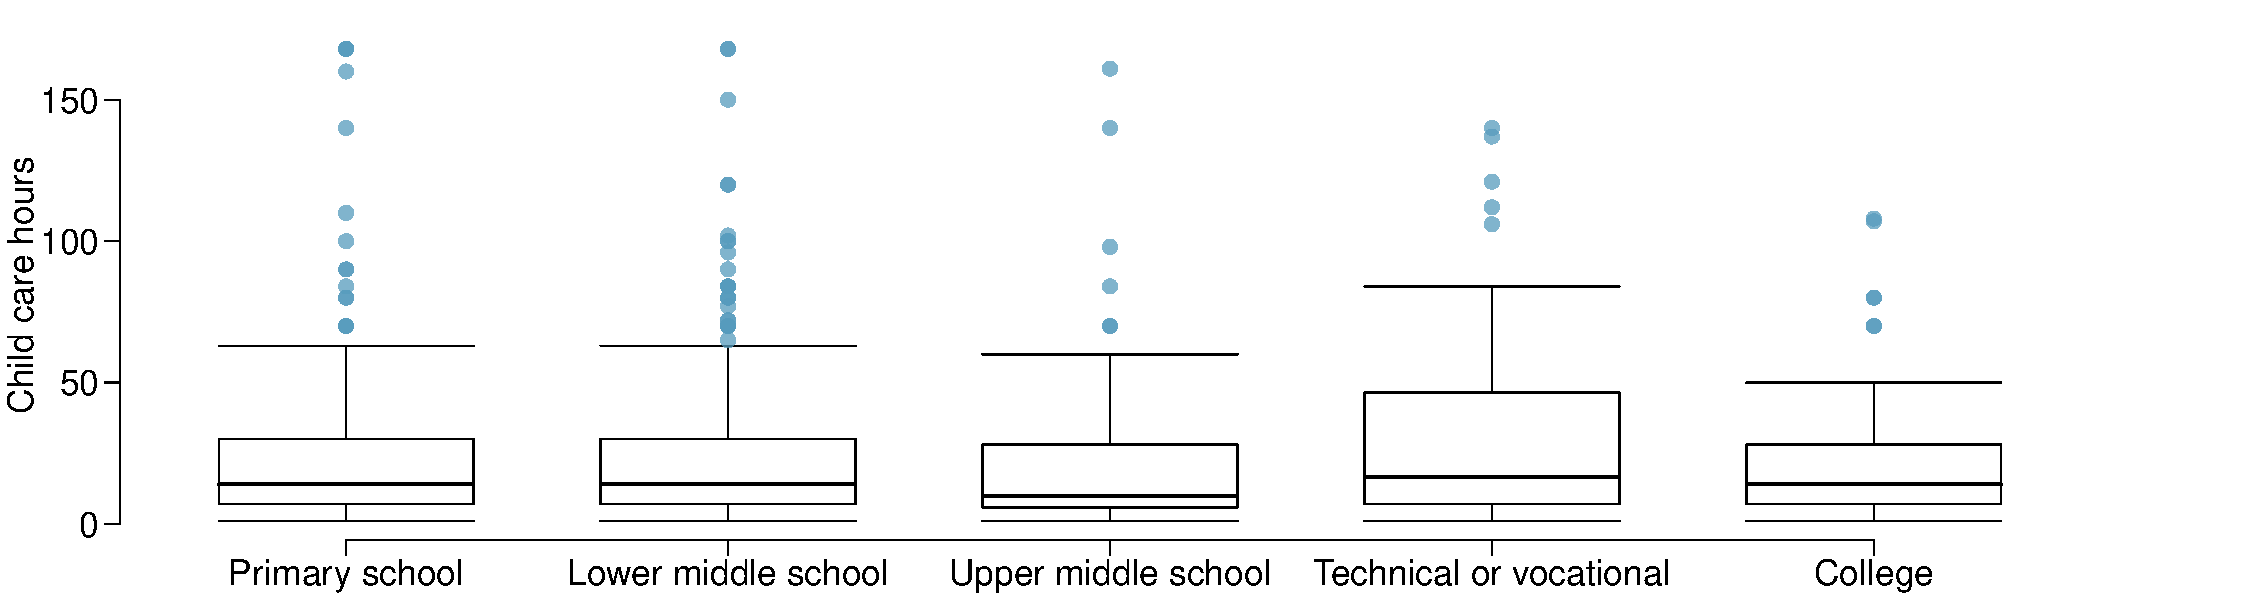
\includegraphics[width=\textwidth]{ch_inference_for_means/figures/eoce/child_care_hours/child_care_hours.pdf}
\end{center}
\begin{center}
\begin{tabular}{lrrrrr}
\hline
            & Df    & Sum Sq    & Mean Sq   & F value   & Pr($>$F) \\ 
\hline
education   & 4     & 4142.09   & 1035.52   & 1.26      & 0.2846 \\ 
Residuals   & 794   & 653047.83 & 822.48    &           &  \\ 
\hline
\end{tabular}
\end{center}
\begin{parts}
\item Write the hypotheses for testing for a difference between the average 
number of hours spent on child care across educational attainment levels.
\item What is the conclusion of the hypothesis test?
\end{parts}
}{}

% 11

\eoce{\qt{Prison isolation experiment, Part II\label{prison_isolation_anova}} Exercise~\ref{prison_isolation_T} introduced an experiment that was conducted with the goal of identifying a treatment that reduces subjects' psychopathic deviant T scores, where this score measures a person's need for control or his rebellion against control. In Exercise~\ref{prison_isolation_T} you evaluated the success of each treatment individually. An alternative analysis involves comparing the success of treatments. The relevant ANOVA output is given below.
\begin{center}
\begin{tabular}{lrrrrr}
  \hline
 & Df & Sum Sq & Mean Sq & F value & Pr($>$F) \\ 
  \hline
treatment & 2 & 639.48 & 319.74 & 3.33 & 0.0461 \\ 
  Residuals & 39 & 3740.43 & 95.91 &  &  \\ 
   \hline
\multicolumn{6}{r}{$s_{pooled} = 9.793$ on $df=39$}
\end{tabular}
\end{center}
\begin{parts}
\item What are the hypotheses?
\item What is the conclusion of the test? Use a 5\% significance level.
\item If in part~(b) you determined that the test is significant, conduct pairwise tests to determine which groups are different from each other. If you did not reject the null hypothesis in part~(b), recheck your answer.
\end{parts}
}{}

% 12

\eoce{\qt{True / False: ANOVA, Part II\label{tf_anova_2}} Determine if the following statements are true or false, and explain your reasoning for statements you identify as false.

If the null hypothesis that the means of four groups are all the same is rejected using ANOVA at a 5\% significance level, then ...
\begin{parts}
\item we can then conclude that all the means are different from one another.
\item the standardized variability between groups is higher than the standardized variability within groups.
\item the pairwise analysis will identify at least one pair of means that are significantly different.
\item the appropriate $\alpha$ to be used in pairwise comparisons is 0.05 / 4 = 0.0125 since there are four groups.
\end{parts}
}{}
